\documentclass[linenumbers]{aastex631}

%% The default is a single spaced, 10 point font, single spaced article.
%% There are 5 other style options available via an optional argument. They
%% can be invoked like this:
%%
%% \documentclass[arguments]{aastex631}
%% 
%% where the layout options are:
%%
%%  twocolumn   : two text columns, 10 point font, single spaced article.
%%                This is the most compact and represent the final published
%%                derived PDF copy of the accepted manuscript from the publisher
%%  manuscript  : one text column, 12 point font, double spaced article.
%%  preprint    : one text column, 12 point font, single spaced article.  
%%  preprint2   : two text columns, 12 point font, single spaced article.
%%  modern      : a stylish, single text column, 12 point font, article with
%% 		  wider left and right margins. This uses the Daniel
%% 		  Foreman-Mackey and David Hogg design.
%%  RNAAS       : Supresses an abstract. Originally for RNAAS manuscripts 
%%                but now that abstracts are required this is obsolete for
%%                AAS Journals. Authors might need it for other reasons. DO NOT
%%                use \begin{abstract} and \end{abstract} with this style.
%%
%% Note that you can submit to the AAS Journals in any of these 6 styles.
%%
%% There are other optional arguments one can invoke to allow other stylistic
%% actions. The available options are:
%%
%%   astrosymb    : Loads Astrosymb font and define \astrocommands. 
%%   tighten      : Makes baselineskip slightly smaller, only works with 
%%                  the twocolumn substyle.
%%   times        : uses times font instead of the default
%%   linenumbers  : turn on lineno package.
%%   trackchanges : required to see the revision mark up and print its output
%%   longauthor   : Do not use the more compressed footnote style (default) for 
%%                  the author/collaboration/affiliations. Instead print all
%%                  affiliation information after each name. Creates a much 
%%                  longer author list but may be desirable for short 
%%                  author papers.
%% twocolappendix : make 2 column appendix.
%%   anonymous    : Do not show the authors, affiliations and acknowledgments 
%%                  for dual anonymous review.
%%
%% these can be used in any combination, e.g.
%%
%% \documentclass[twocolumn,linenumbers,trackchanges]{aastex631}
%%
%% AASTeX v6.* now includes \hyperref support. While we have built in specific
%% defaults into the classfile you can manually override them with the
%% \hypersetup command. For example,
%%
%% \hypersetup{linkcolor=red,citecolor=green,filecolor=cyan,urlcolor=magenta}
%%
%% will change the color of the internal links to red, the links to the
%% bibliography to green, the file links to cyan, and the external links to
%% magenta. Additional information on \hyperref options can be found here:
%% https://www.tug.org/applications/hyperref/manual.html#x1-40003
%%

\usepackage{amsmath, hyperref, gensymb}

\newcommand{\vdag}{(v)^\dagger}
\newcommand\aastex{AAS\TeX}
\newcommand\latex{La\TeX}

%% Reintroduced the \received and \accepted commands from AASTeX v5.2
%\received{March 1, 2021}
%\revised{April 1, 2021}
%\accepted{\today}

%% Command to document which AAS Journal the manuscript was submitted to.
%% Adds "Submitted to " the argument.
%\submitjournal{PSJ}

%\graphicspath{{./}{figures/}}
%% This is the end of the preamble.  Indicate the beginning of the
%% manuscript itself with \begin{document}.

\begin{document}

\title{Three Point Correlation signals of PSF aberrations}

\author[0000-0003-2429-5811]{Shubh Agrawal}
\affiliation{University of Pennsylvania}

\begin{abstract}
\href{https://github.com/shubhagrawal30/aberrations}{GitHub}
\end{abstract}

\keywords{}

\section{Shear from Zernike coefficients} \label{sec:ell_zernike} 

We use Section 5.1 of \cite{jarvis_telescope_2008} to write down our aberration model, along with Section 10.3 of \cite{dodelson_modern_2003} to write down the ellipticity and shear in terms of PSF shape and size: 

\begin{equation}
d, a, c, s \xrightarrow{\text{\cite{jarvis_telescope_2008}}} Q(x, y), S(x, y) \xrightarrow{\text{\cite{dodelson_modern_2003}}} \gamma_1, \gamma_2
\end{equation}

Coefficients of the Zernike polynomials are field-of-view dependent and can be parameterized by position $x, y$ on the sky. We consider contributions from the first few dominant coefficients and define the following:
\begin{align}
d &= A_\text{defocus} \\
a &= A_\text{astigmation-c} + i A_\text{astigmation-s} \\
c &= A_\text{coma-c} + i A_\text{coma-s} \\
s &= A_\text{spherical}
\end{align}

The shape and size of the PSF are then given respectively as:
\begin{align}
Q(X, Y) &= \frac{\int dx dy I(x, y) (x+iy)^2}{\int dx dy I(x, y)} = 4 \Big(d+\frac{4}{3}s \Big) a + \frac{1}{3} c^2\\
S(X, Y) &= \frac{\int dx dy I(x, y) |x+iy|^2}{\int dx dy I(x, y)} = 2 \Big(d+\frac{4}{3}s \Big)^2 + 2 |a|^2 + \frac{2}{3} |c|^2 + \frac{4}{9} s^2\\
\end{align}
with the integral centered at $X, Y$. 

Ellipticity $\epsilon = \epsilon_1 + i \epsilon_2$ can be written as:
\begin{align}
\epsilon = \epsilon_1 + i \epsilon_2 &= \frac{q_{xx} - q_{yy}}{q_{xx} + q_{yy}} + i \frac{2 q_{xy}}{q_{xx} + q_{yy}}\\
&= \frac{1}{\int dx dy I(x, y) (x^2 + y^2)} \int dx dy I(x, y) \Big( x^2 + i^2 y^2 + 2ixy \Big) \\
&= Q \Big/ S
\end{align}

In the weak lensing limit, 
\begin{align}
\gamma_1 = \Re(Q / S) \Big/ 2 && \gamma_2 = \Im(Q / S) \Big/ 2
\end{align}

\newpage
\section{Toy Models} \label{sec:toy_models}

\subsection{Constant coefficients}

\begin{align}
d &= 10^{-1} \\
s &= 10^{-2} \\
a &= 10^{-2} + i \times 3 \times 10^{-3} \\
c &= 10^{-2} + i \times 3 \times 10^{-3}
\end{align}

\begin{figure}[h]
\centering
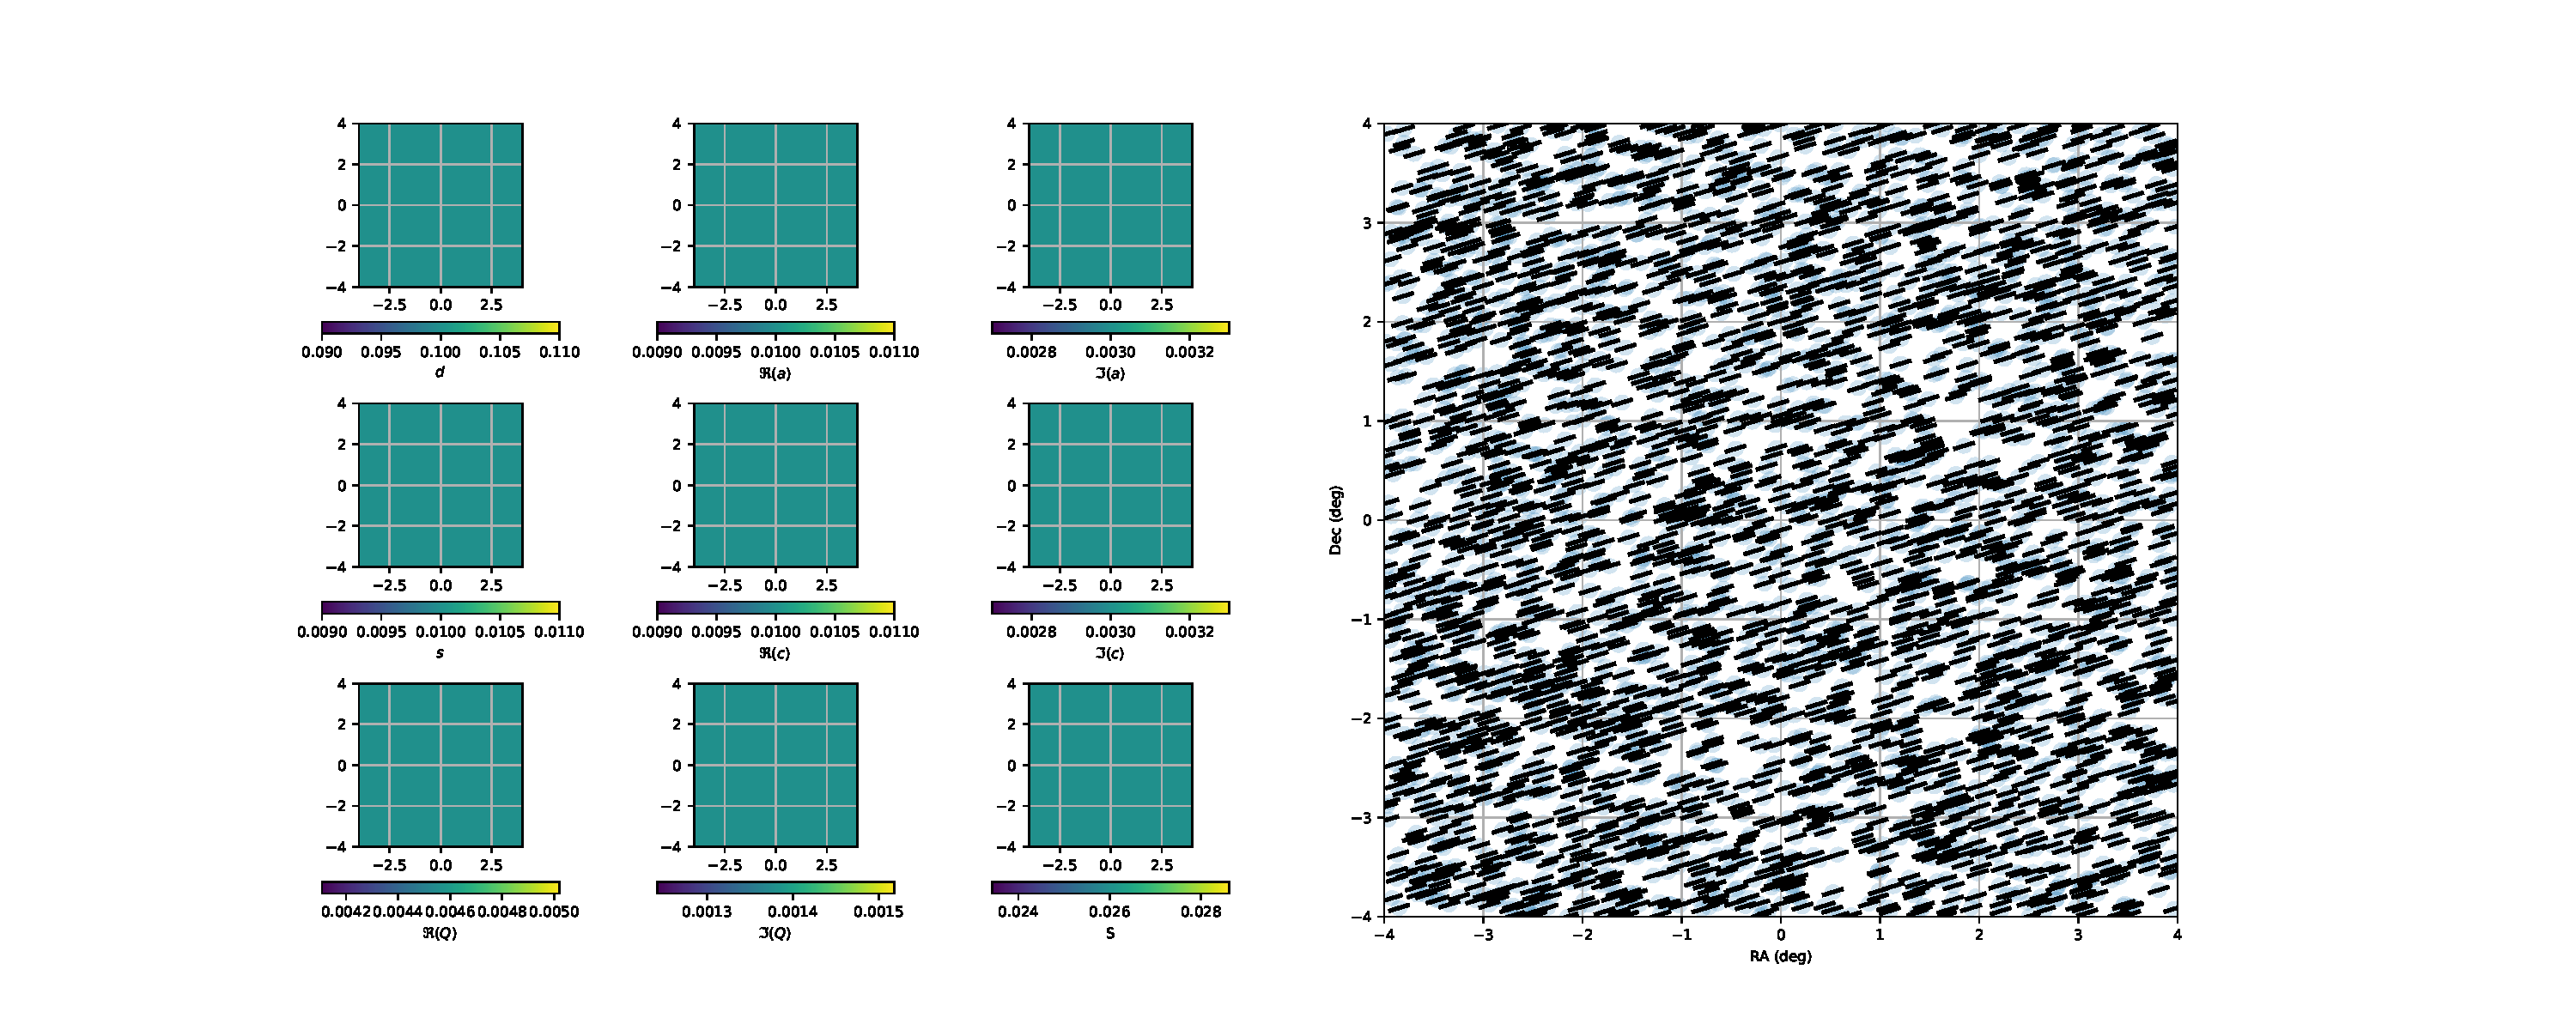
\includegraphics[width=\textwidth]{figs/20230109_constant/coeff_shear.pdf}
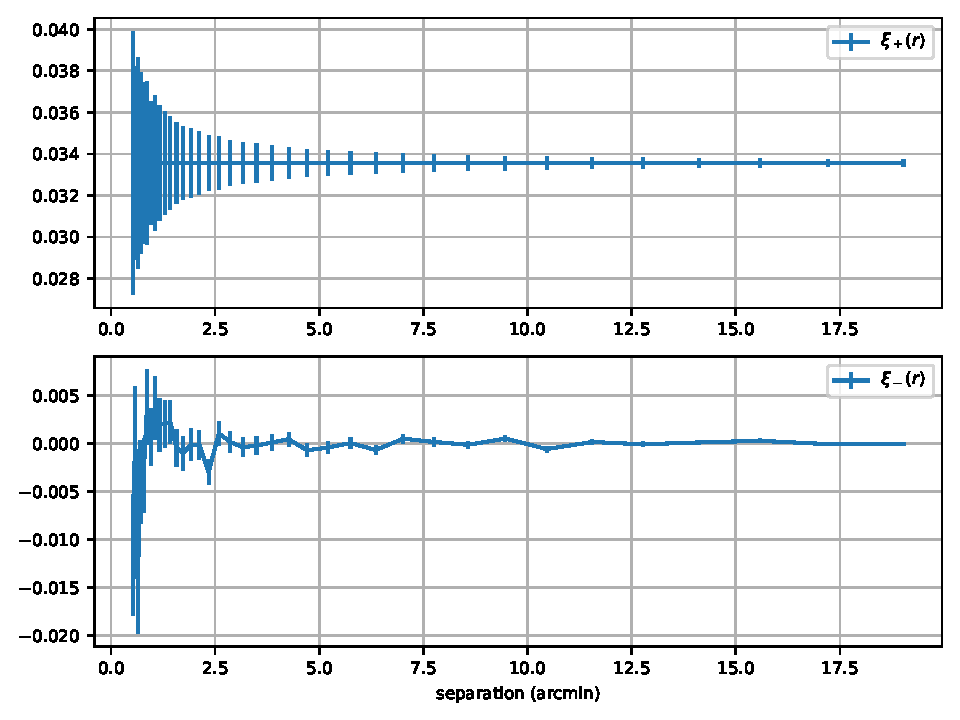
\includegraphics[width=0.48\textwidth]{figs/20230109_constant/2point.pdf}
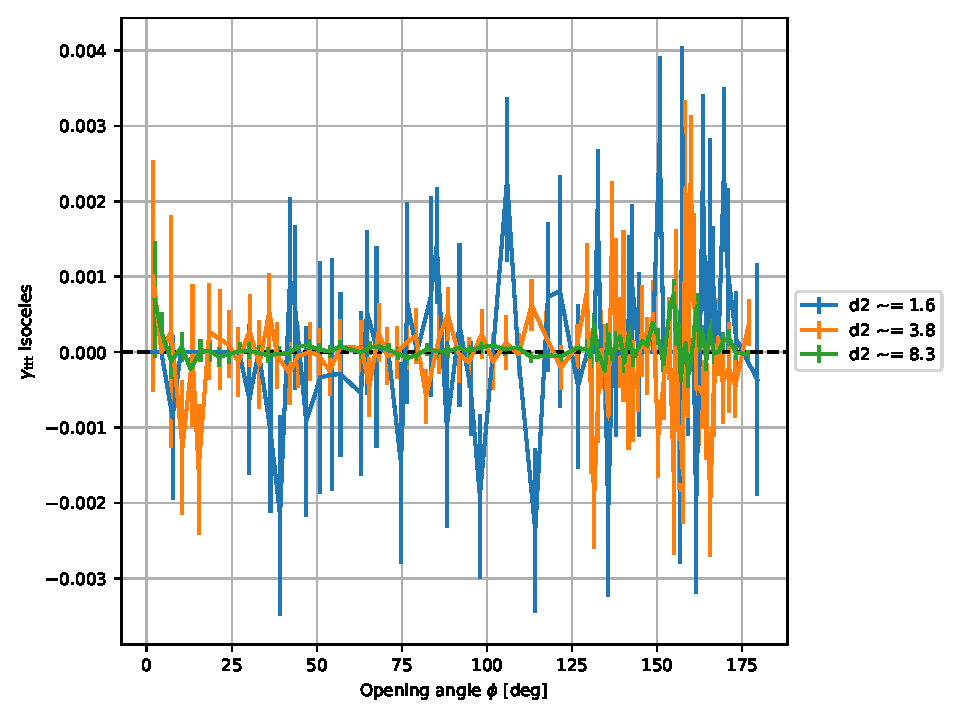
\includegraphics[width=0.48\textwidth]{figs/20230109_constant/3point.pdf}
\caption{Constant coefficients.}
\label{fig:constant}
\end{figure}

\newpage
\subsection{Radial dependence on imaginary parts}

\begin{align}
d &= 10^{-1} \\
s &= 10^{-2} \\
a &= 10^{-2} + i \times 3 \times 10^{-3} (x^2+y^2) \\
c &= 10^{-2} + i \times 3 \times 10^{-3} (x^2+y^2)
\end{align}

\begin{figure}[h]
\centering
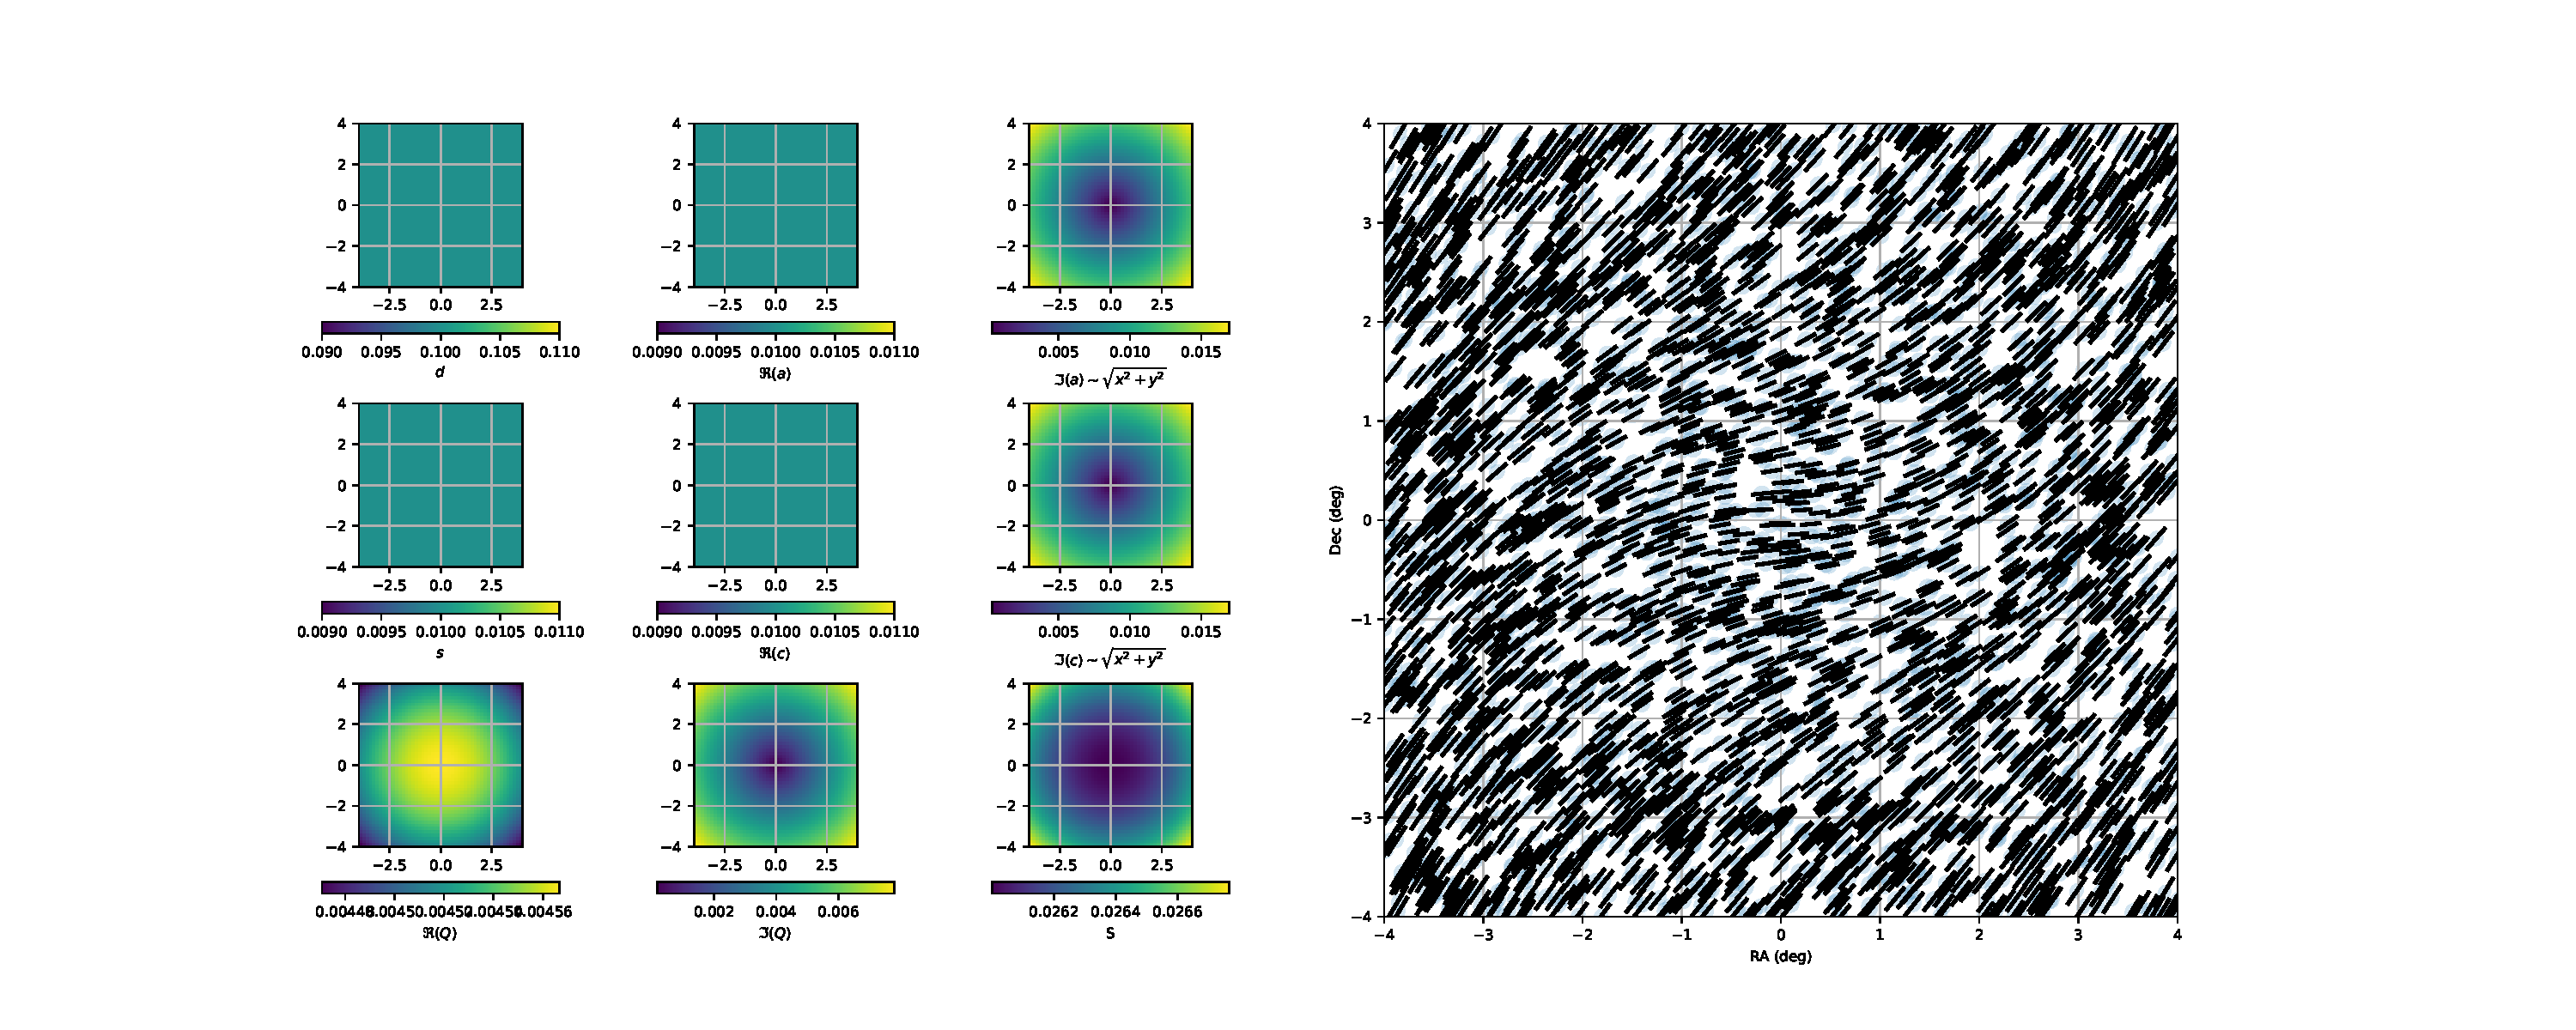
\includegraphics[width=\textwidth]{figs/20230109_radial_imag/coeff_shear.pdf}
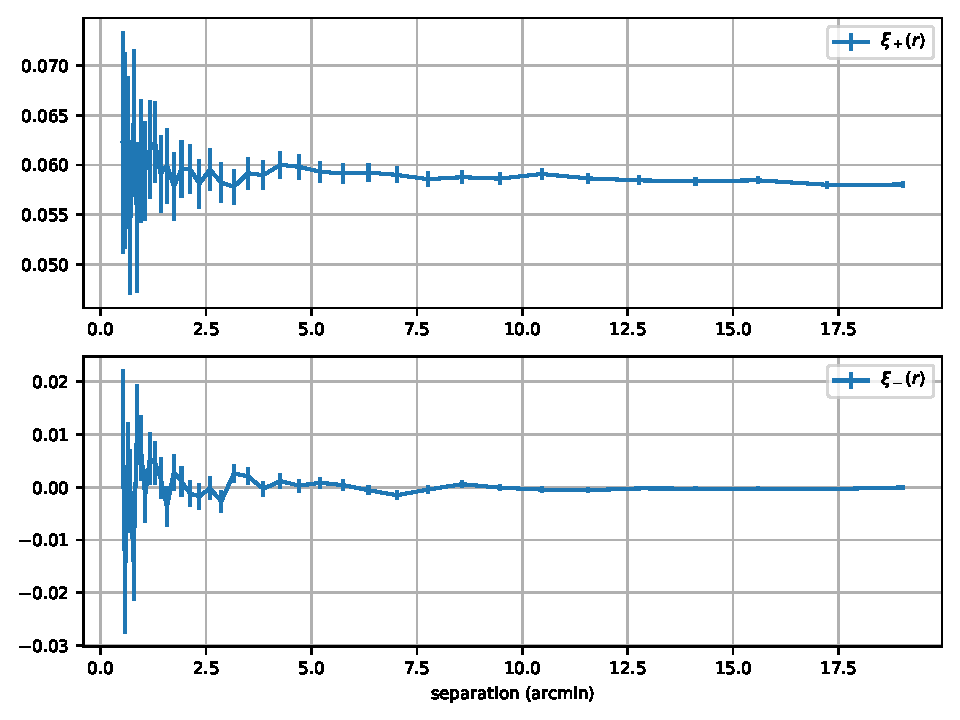
\includegraphics[width=0.48\textwidth]{figs/20230109_radial_imag/2point.pdf}
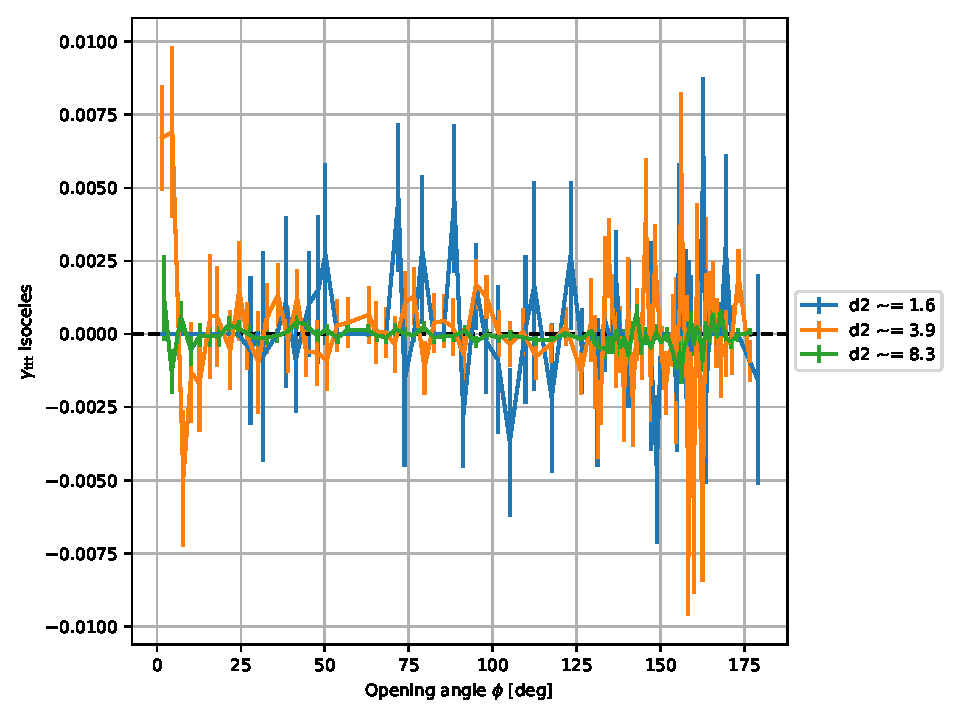
\includegraphics[width=0.48\textwidth]{figs/20230109_radial_imag/3point.pdf}
\caption{Radial coefficients.}
\label{fig:radial}
\end{figure}

% \documentclass[linenumbers]{aastex631}

%% The default is a single spaced, 10 point font, single spaced article.
%% There are 5 other style options available via an optional argument. They
%% can be invoked like this:
%%
%% \documentclass[arguments]{aastex631}
%% 
%% where the layout options are:
%%
%%  twocolumn   : two text columns, 10 point font, single spaced article.
%%                This is the most compact and represent the final published
%%                derived PDF copy of the accepted manuscript from the publisher
%%  manuscript  : one text column, 12 point font, double spaced article.
%%  preprint    : one text column, 12 point font, single spaced article.  
%%  preprint2   : two text columns, 12 point font, single spaced article.
%%  modern      : a stylish, single text column, 12 point font, article with
%% 		  wider left and right margins. This uses the Daniel
%% 		  Foreman-Mackey and David Hogg design.
%%  RNAAS       : Supresses an abstract. Originally for RNAAS manuscripts 
%%                but now that abstracts are required this is obsolete for
%%                AAS Journals. Authors might need it for other reasons. DO NOT
%%                use \begin{abstract} and \end{abstract} with this style.
%%
%% Note that you can submit to the AAS Journals in any of these 6 styles.
%%
%% There are other optional arguments one can invoke to allow other stylistic
%% actions. The available options are:
%%
%%   astrosymb    : Loads Astrosymb font and define \astrocommands. 
%%   tighten      : Makes baselineskip slightly smaller, only works with 
%%                  the twocolumn substyle.
%%   times        : uses times font instead of the default
%%   linenumbers  : turn on lineno package.
%%   trackchanges : required to see the revision mark up and print its output
%%   longauthor   : Do not use the more compressed footnote style (default) for 
%%                  the author/collaboration/affiliations. Instead print all
%%                  affiliation information after each name. Creates a much 
%%                  longer author list but may be desirable for short 
%%                  author papers.
%% twocolappendix : make 2 column appendix.
%%   anonymous    : Do not show the authors, affiliations and acknowledgments 
%%                  for dual anonymous review.
%%
%% these can be used in any combination, e.g.
%%
%% \documentclass[twocolumn,linenumbers,trackchanges]{aastex631}
%%
%% AASTeX v6.* now includes \hyperref support. While we have built in specific
%% defaults into the classfile you can manually override them with the
%% \hypersetup command. For example,
%%
%% \hypersetup{linkcolor=red,citecolor=green,filecolor=cyan,urlcolor=magenta}
%%
%% will change the color of the internal links to red, the links to the
%% bibliography to green, the file links to cyan, and the external links to
%% magenta. Additional information on \hyperref options can be found here:
%% https://www.tug.org/applications/hyperref/manual.html#x1-40003
%%
%% Note that in v6.3 "bookmarks" has been changed to "true" in hyperref
%% to improve the accessibility of the compiled pdf file.
%%
%% If you want to create your own macros, you can do so
%% using \newcommand. Your macros should appear before
%% the \begin{document} command.
%%
\newcommand{\vdag}{(v)^\dagger}
\newcommand\aastex{AAS\TeX}
\newcommand\latex{La\TeX}

%% Reintroduced the \received and \accepted commands from AASTeX v5.2
%\received{March 1, 2021}
%\revised{April 1, 2021}
%\accepted{\today}

%% Command to document which AAS Journal the manuscript was submitted to.
%% Adds "Submitted to " the argument.
%\submitjournal{PSJ}

%% For manuscript that include authors in collaborations, AASTeX v6.31
%% builds on the \collaboration command to allow greater freedom to 
%% keep the traditional author+affiliation information but only show
%% subsets. The \collaboration command now must appear AFTER the group
%% of authors in the collaboration and it takes TWO arguments. The last
%% is still the collaboration identifier. The text given in this
%% argument is what will be shown in the manuscript. The first argument
%% is the number of author above the \collaboration command to show with
%% the collaboration text. If there are authors that are not part of any
%% collaboration the \nocollaboration command is used. This command takes
%% one argument which is also the number of authors above to show. A
%% dashed line is shown to indicate no collaboration. This example manuscript
%% shows how these commands work to display specific set of authors 
%% on the front page.
%%
%% For manuscript without any need to use \collaboration the 
%% \AuthorCollaborationLimit command from v6.2 can still be used to 
%% show a subset of authors.
%
%\AuthorCollaborationLimit=2
%
%% will only show Schwarz & Muench on the front page of the manuscript
%% (assuming the \collaboration and \nocollaboration commands are
%% commented out).
%%
%% Note that all of the author will be shown in the published article.
%% This feature is meant to be used prior to acceptance to make the
%% front end of a long author article more manageable. Please do not use
%% this functionality for manuscripts with less than 20 authors. Conversely,
%% please do use this when the number of authors exceeds 40.
%%
%% Use \allauthors at the manuscript end to show the full author list.
%% This command should only be used with \AuthorCollaborationLimit is used.

%% The following command can be used to set the latex table counters.  It
%% is needed in this document because it uses a mix of latex tabular and
%% AASTeX deluxetables.  In general it should not be needed.
%\setcounter{table}{1}

%%%%%%%%%%%%%%%%%%%%%%%%%%%%%%%%%%%%%%%%%%%%%%%%%%%%%%%%%%%%%%%%%%%%%%%%%%%%%%%%
%%
%% The following section outlines numerous optional output that
%% can be displayed in the front matter or as running meta-data.
%%
%% If you wish, you may supply running head information, although
%% this information may be modified by the editorial offices.
%\shorttitle{AASTeX v6.3.1 Sample article}
%\shortauthors{Schwarz et al.}
%%
%% You can add a light gray and diagonal water-mark to the first page 
%% with this command:
%% \watermark{text}
%% where "text", e.g. DRAFT, is the text to appear.  If the text is 
%% long you can control the water-mark size with:
%% \setwatermarkfontsize{dimension}
%% where dimension is any recognized LaTeX dimension, e.g. pt, in, etc.
%%
%%%%%%%%%%%%%%%%%%%%%%%%%%%%%%%%%%%%%%%%%%%%%%%%%%%%%%%%%%%%%%%%%%%%%%%%%%%%%%%%
%\graphicspath{{./}{figures/}}
%% This is the end of the preamble.  Indicate the beginning of the
%% manuscript itself with \begin{document}.

\begin{document}

\title{Template \aastex Article with Examples: 
v6.3.1\footnote{Released on March, 1st, 2021}}

%% LaTeX will automatically break titles if they run longer than
%% one line. However, you may use \\ to force a line break if
%% you desire. In v6.31 you can include a footnote in the title.

%% A significant change from earlier AASTEX versions is in the structure for 
%% calling author and affiliations. The change was necessary to implement 
%% auto-indexing of affiliations which prior was a manual process that could 
%% easily be tedious in large author manuscripts.
%%
%% The \author command is the same as before except it now takes an optional
%% argument which is the 16 digit ORCID. The syntax is:
%% \author[xxxx-xxxx-xxxx-xxxx]{Author Name}
%%
%% This will hyperlink the author name to the author's ORCID page. Note that
%% during compilation, LaTeX will do some limited checking of the format of
%% the ID to make sure it is valid. If the "orcid-ID.png" image file is 
%% present or in the LaTeX pathway, the OrcID icon will appear next to
%% the authors name.
%%
%% Use \affiliation for affiliation information. The old \affil is now aliased
%% to \affiliation. AASTeX v6.31 will automatically index these in the header.
%% When a duplicate is found its index will be the same as its previous entry.
%%
%% Note that \altaffilmark and \altaffiltext have been removed and thus 
%% can not be used to document secondary affiliations. If they are used latex
%% will issue a specific error message and quit. Please use multiple 
%% \affiliation calls for to document more than one affiliation.
%%
%% The new \altaffiliation can be used to indicate some secondary information
%% such as fellowships. This command produces a non-numeric footnote that is
%% set away from the numeric \affiliation footnotes.  NOTE that if an
%% \altaffiliation command is used it must come BEFORE the \affiliation call,
%% right after the \author command, in order to place the footnotes in
%% the proper location.
%%
%% Use \email to set provide email addresses. Each \email will appear on its
%% own line so you can put multiple email address in one \email call. A new
%% \correspondingauthor command is available in V6.31 to identify the
%% corresponding author of the manuscript. It is the author's responsibility
%% to make sure this name is also in the author list.
%%
%% While authors can be grouped inside the same \author and \affiliation
%% commands it is better to have a single author for each. This allows for
%% one to exploit all the new benefits and should make book-keeping easier.
%%
%% If done correctly the peer review system will be able to
%% automatically put the author and affiliation information from the manuscript
%% and save the corresponding author the trouble of entering it by hand.

%\correspondingauthor{August Muench}
%\email{greg.schwarz@aas.org, gus.muench@aas.org}

\author[0000-0002-0786-7307]{Greg J. Schwarz}
\affiliation{American Astronomical Society \\
1667 K Street NW, Suite 800 \\
Washington, DC 20006, USA}

\author{August Muench}
\affiliation{American Astronomical Society \\
1667 K Street NW, Suite 800 \\
Washington, DC 20006, USA}

\collaboration{20}{(AAS Journals Data Editors)}

\author{F.X Timmes}
\affiliation{Arizona State University}
\affiliation{AAS Journals Associate Editor-in-Chief}

\author{Amy Hendrickson}
\altaffiliation{AASTeX v6+ programmer}
\affiliation{TeXnology Inc.}

\author{Julie Steffen}
\affiliation{AAS Director of Publishing}
\affiliation{American Astronomical Society \\
1667 K Street NW, Suite 800 \\
Washington, DC 20006, USA}

%% Note that the \and command from previous versions of AASTeX is now
%% depreciated in this version as it is no longer necessary. AASTeX 
%% automatically takes care of all commas and "and"s between authors names.

%% AASTeX 6.31 has the new \collaboration and \nocollaboration commands to
%% provide the collaboration status of a group of authors. These commands 
%% can be used either before or after the list of corresponding authors. The
%% argument for \collaboration is the collaboration identifier. Authors are
%% encouraged to surround collaboration identifiers with ()s. The 
%% \nocollaboration command takes no argument and exists to indicate that
%% the nearby authors are not part of surrounding collaborations.

%% Mark off the abstract in the ``abstract'' environment. 
\begin{abstract}

This example manuscript is intended to serve as a tutorial and template for
authors to use when writing their own AAS Journal articles. The manuscript
includes a history of \aastex\ and includes figure and table examples to illustrate these features. Information on features not explicitly mentioned in the article can be viewed in the manuscript comments or more extensive online
documentation. Authors are welcome replace the text, tables, figures, and
bibliography with their own and submit the resulting manuscript to the AAS
Journals peer review system.  The first lesson in the tutorial is to remind
authors that the AAS Journals, the Astrophysical Journal (ApJ), the
Astrophysical Journal Letters (ApJL), the Astronomical Journal (AJ), and
the Planetary Science Journal (PSJ) all have a 250 word limit for the 
abstract\footnote{Abstracts for Research Notes of the American Astronomical 
Society (RNAAS) are limited to 150 words}.  If you exceed this length the
Editorial office will ask you to shorten it. This abstract has 161 words.

\end{abstract}

%% Keywords should appear after the \end{abstract} command. 
%% The AAS Journals now uses Unified Astronomy Thesaurus concepts:
%% https://astrothesaurus.org
%% You will be asked to selected these concepts during the submission process
%% but this old "keyword" functionality is maintained in case authors want
%% to include these concepts in their preprints.
\keywords{Classical Novae (251) --- Ultraviolet astronomy(1736) --- History of astronomy(1868) --- Interdisciplinary astronomy(804)}

%% From the front matter, we move on to the body of the paper.
%% Sections are demarcated by \section and \subsection, respectively.
%% Observe the use of the LaTeX \label
%% command after the \subsection to give a symbolic KEY to the
%% subsection for cross-referencing in a \ref command.
%% You can use LaTeX's \ref and \label commands to keep track of
%% cross-references to sections, equations, tables, and figures.
%% That way, if you change the order of any elements, LaTeX will
%% automatically renumber them.
%%
%% We recommend that authors also use the natbib \citep
%% and \citet commands to identify citations.  The citations are
%% tied to the reference list via symbolic KEYs. The KEY corresponds
%% to the KEY in the \bibitem in the reference list below. 

\section{Introduction} \label{sec:intro}

\latex\ \footnote{\url{http://www.latex-project.org/}} is a document markup
language that is particularly well suited for the publication of
mathematical and scientific articles \citep{lamport94}. \latex\ was written
in 1985 by Leslie Lamport who based it on the \TeX\ typesetting language
which itself was created by Donald E. Knuth in 1978.  In 1988 a suite of
\latex\ macros were developed to investigate electronic submission and
publication of AAS Journal articles \citep{1989BAAS...21..780H}.  Shortly
afterwards, Chris Biemesdefer merged these macros and more into a \latex\
2.08 style file called \aastex.  These early \aastex\ versions introduced
many common commands and practices that authors take for granted today.
Substantial revisions
were made by Lee Brotzman and Pierre Landau when the package was updated to
v4.0.  AASTeX v5.0, written in 1995 by Arthur Ogawa, upgraded to \latex\ 2e
which uses the document class in lieu of a style file.  Other improvements
to version 5 included hypertext support, landscape deluxetables and
improved figure support to facilitate electronic submission.  
\aastex\ v5.2 was released in 2005 and introduced additional graphics
support plus new mark up to identifier astronomical objects, datasets and
facilities.

In 1996 Maxim Markevitch modified the AAS preprint style file, aaspp4.sty,
to closely emulate the very tight, two column style of a typeset
Astrophysical Journal article.  The result was emulateapj.sty.  A year
later Alexey Vikhlinin took over development and maintenance.  In 2001 he
converted emulateapj into a class file in \latex\ 2e and in 2003 Vikhlinin
completely rewrote emulateapj based on the APS Journal's RevTEX class.

During this time emulateapj gained growing acceptance in the astronomical
community as it filled an author need to obtain an approximate number of
manuscript pages prior to submission for cost and length estimates. The
tighter typeset also had the added advantage of saving paper when printing
out hard copies.

Even though author publication charges are no longer based on print pages
\footnote{see Section \ref{sec:pubcharge} in the Appendix for more details
about how current article costs are calculated.} the emulateapj class file
has proven to be extremely popular with AAS Journal authors.  An 
analysis of submitted \latex\ manuscripts in 2015 revealed that $\sim$65\%
either called emulateapj or have a commented emulateapj classfile call
indicating it was used at some stage of the manuscript construction.
Clearly authors want to have access to a tightly typeset version of the
article when corresponding with co-authors and for preprint submissions.

When planning the next \aastex\ release the popularity of emulateapj played
an important roll in the decision to drop the old base code and adopt and
modify emulateapj for \aastex\ v6.+ instead.  The change brings \aastex\
inline with what the majority of authors are already using while still
delivering new and improved features.  \aastex\ v6.0 through v6.31 were
written by Amy Hendrickson. The release dates were January 2016 (v6.0),
October 2016 (v6.1), January 2018 (v6.2), June 2019 (v6.3), and March 2020
(v6.31) respectively.

The rest of this article provides information and examples on how to create
your own AAS Journal manuscript with v6.31. The next section describes
the different manuscript styles available and how they differ from past
releases.  Section \ref{sec:floats} describes table and figure placement. 
Specific examples of a table, Section \ref{subsec:tables}, and a figure,
Section \ref{subsec:figures}, are also provided.  The last section,
\ref{sec:cite}, shows how recognize software and external data as first
class references in the manuscript bibliography.  An appendix is included
for additional information readers might find useful.
More documentation is embedded in the comments of this \latex\ file and in the online documentation at
\url{http://journals.aas.org/authors/aastex.html}.

\section{Manuscript styles} \label{sec:style}

The default style in \aastex\ v6.31 is a tight single column style, e.g. 10
point font, single spaced.  The single column style is very useful for
article with wide equations. It is also the easiest to style to work with
since figures and tables, see Section \ref{sec:floats}, will span the
entire page, reducing the need for address float sizing.

To invoke a two column style similar to the what is produced in
the published PDF copy use \\

\noindent {\tt\string\documentclass[twocolumn]\{aastex631\}}. \\

\noindent Note that in the two column style figures and tables will only
span one column unless specifically ordered across both with the ``*'' flag,
e.g. \\

\noindent{\tt\string\begin\{figure*\}} ... {\tt\string\end\{figure*\}}, \\
\noindent{\tt\string\begin\{table*\}} ... {\tt\string\end\{table*\}}, and \\
\noindent{\tt\string\begin\{deluxetable*\}} ... {\tt\string\end\{deluxetable*\}}. \\

\noindent This option is ignored in the onecolumn style.

Some other style options are outlined in the commented sections of this 
article.  Any combination of style options can be used.

Authors are required to provide line numbering in the manuscript. Line numbering makes it easier for the review to references specific places in the manuscript.
This functionality has been built into AASTeX since v6.0.  The {\tt\string linenumbers} style option invokes the lineno style file to number each article line in the left margin.

There is also a new {\tt\string modern} option that uses a Daniel
Foreman-Mackey and David Hogg design to produce stylish, single column
output that has wider left and right margins. It is designed to have fewer
words per line to improve reader retention. It also looks better on devices
with smaller displays such as smart phones.

The {\tt\string anonymous} option will prevent the author and affiliations
from being shown in the compiled pdf copy. This option allows the author 
to keep this critical information in the latex file but prevent the reviewer
from seeing it during peer review if dual anonymous review (DAR) is requested. 
Likewise, acknowledgments can also be hidden if placed in the new 
{\tt\string\begin\{acknowledgments\}} ... {\tt\string\end\{acknowledgments\}}
environment. The use of this option is highly recommended for PSJ submissions. 
Advice for anonymizing your manuscript for DAR is provided at 
\url{https://journals.aas.org/manuscript-preparation/#dar}.

\section{Floats} \label{sec:floats}

Floats are non-text items that generally can not be split over a page.
They also have captions and can be numbered for reference.  Primarily these
are figures and tables but authors can define their own. \latex\ tries to
place a float where indicated in the manuscript but will move it later if
there is not enough room at that location, hence the term ``float''.

Authors are encouraged to embed their tables and figures within the text as
they are mentioned.  Please do not place the figures and text at the end of
the article as was the old practice.  Editors and the vast majority of
referees find it much easier to read a manuscript with embedded figures and
tables.

Depending on the number of floats and the particular amount of text and
equations present in a manuscript the ultimate location of any specific
float can be hard to predict prior to compilation. It is recommended that
authors textbf{not} spend significant time trying to get float placement
perfect for peer review.  The AAS Journal's publisher has sophisticated
typesetting software that will produce the optimal layout during
production.

Note that authors of Research Notes are only allowed one float, either one
table or one figure.

For authors that do want to take the time to optimize the locations of
their floats there are some techniques that can be used.  The simplest
solution is to placing a float earlier in the text to get the position
right but this option will break down if the manuscript is altered.
A better method is to force \latex\ to place a
float in a general area with the use of the optional {\tt\string [placement
specifier]} parameter for figures and tables. This parameter goes after
{\tt\string \begin\{figure\}}, {\tt\string \begin\{table\}}, and
{\tt\string \begin\{deluxetable\}}.  The main arguments the specifier takes
are ``h'', ``t'', ``b'', and ``!''.  These tell \latex\ to place the float
\underline{h}ere (or as close as possible to this location as possible), at
the \underline{t}op of the page, and at the \underline{b}ottom of the page.
The last argument, ``!'', tells \latex\ to override its internal method of
calculating the float position.  A sequence of rules can be created by
using multiple arguments.  For example, {\tt\string \begin\{figure\}[htb!]}
tells \latex\ to try the current location first, then the top of the page
and finally the bottom of the page without regard to what it thinks the
proper position should be.  Many of the tables and figures in this article
use a placement specifier to set their positions.

Note that the \latex\ {\tt\string tabular} environment is not a float.  Only
when a {\tt\string tabular} is surrounded by {\tt\string\begin\{table\}} ...
{\tt\string\end\{table\}} is it a true float and the rules and suggestions
above apply.

In AASTeX v6.31 all deluxetables are float tables and thus if they are
longer than a page will spill off the bottom. Long deluxetables should
begin with the {\tt\string\startlongtable} command. This initiates a
longtable environment.  Authors might have to use {\tt\string\clearpage} to
isolate a long table or optimally place it within the surrounding text.

\subsection{Tables} \label{subsec:tables}

Tables can be constructed with \latex's standard table environment or the
\aastex's deluxetable environment. The deluxetable construct handles long
tables better but has a larger overhead due to the greater amount of
defined mark up used set up and manipulate the table structure.  The choice
of which to use is up to the author. 

Tables longer than 250 data lines and complex tables should only have a
short example table with the full data set available in the machine
readable format.  The machine readable table will be available in the HTML
version of the article with just a short example in the PDF. Authors are
required to indicate in the table comments that the data in machine 
readable format in the full article.
Authors are encouraged to create their own machine
readable tables using the online tool at
\url{http://authortools.aas.org/MRT/upload.html} but the data editors will review and edit all submissions prior to publication.

Full details on how to create the different types of tables are given in the AASTeX guidelines at \url{http://journals.aas.org/authors/aastex.html}

\subsubsection{Splitting a table into multiple horizontal components}

Since the AAS Journals are now all electronic with no print version there is
no reason why tables can not be as wide as authors need them to be.
However, there are some artificial limitations based on the width of a
print page.  The old way around this limitation was to rotate into 
landscape mode and use the smallest available table font
sizes, e.g. {\tt\string\tablewidth}, to get the table to fit.
Unfortunately, this was not always enough but now there is a new way to break
a table into two or three components so that it flows down a page by
invoking a new table type, splittabular or splitdeluxetable. Within these
tables a new ``B'' column separator is introduced.  Much like the vertical
bar option, ``$\vert$'', that produces a vertical table lines 
the new ``B'' separator indicates where to \underline{B}reak
a table.  Up to two ``B''s may be included.

Table \ref{tab:deluxesplit} 
shows how to split a wide deluxetable into three parts with
the {\tt\string\splitdeluxetable} command.  The {\tt\string\colnumbers}
option is on to show how the automatic column numbering carries through the
second table component.

\begin{splitdeluxetable*}{lccccBcccccBcccc}
\tabletypesize{\scriptsize}
\tablewidth{0pt} 
%\tablenum{1}
\tablecaption{Measurements of Emission Lines: two breaks \label{tab:deluxesplit}}
\tablehead{
\colhead{Model} & \colhead{Component}& \colhead{Shift} & \colhead{FWHM} &
\multicolumn{10}{c}{Flux} \\
\colhead{} & \colhead{} & \colhead{($\rm
km~s^{-1}$)}& \colhead{($\rm km~s^{-1}$)} & \multicolumn{10}{c}{($\rm
10^{-17}~erg~s^{-1}~cm^{-2}$)} \\
\cline{5-14}
\colhead{} & \colhead{} &
\colhead{} & \colhead{} & \colhead{Ly$\alpha$} & \colhead{N\,{\footnotesize
V}} & \colhead{Si\,{\footnotesize IV}} & \colhead{C\,{\footnotesize IV}} &
\colhead{Mg\,{\footnotesize II}} & \colhead{H$\gamma$} & \colhead{H$\beta$}
& \colhead{H$\alpha$} & \colhead{He\,{\footnotesize I}} &
\colhead{Pa$\gamma$}
} 
\colnumbers
\startdata 
{       }& BELs& -97.13 &    9117$\pm      38$&    1033$\pm      33$&$< 35$&$<     166$&     637$\pm      31$&    1951$\pm      26$&     991$\pm 30$&    3502$\pm      42$&   20285$\pm      80$&    2025$\pm     116$& 1289$\pm     107$\\ 
{Model 1}& IELs& -4049.123 & 1974$\pm      22$&    2495$\pm      30$&$<     42$&$<     109$&     995$\pm 186$&      83$\pm      30$&      75$\pm      23$&     130$\pm      25$& 357$\pm      94$&     194$\pm      64$& 36$\pm      23$\\
{       }& NELs& \nodata &     641$\pm       4$&     449$\pm 23$&$<      6$&$<       9$&       --            &     275$\pm      18$& 150$\pm      11$&     313$\pm      12$&     958$\pm      43$&     318$\pm 34$& 151$\pm       17$\\
\hline
{       }& BELs& -85 &    8991$\pm      41$& 988$\pm      29$&$<     24$&$<     173$&     623$\pm      28$&    1945$\pm 29$&     989$\pm      27$&    3498$\pm      37$&   20288$\pm      73$& 2047$\pm     143$& 1376$\pm     167$\\
{Model 2}& IELs& -51000 &    2025$\pm      26$& 2494$\pm      32$&$<     37$&$<     124$&    1005$\pm     190$&      72$\pm 28$&      72$\pm      21$&     113$\pm      18$&     271$\pm      85$& 205$\pm      72$& 34$\pm      21$\\
{       }& NELs& 52 &     637$\pm      10$&     477$\pm 17$&$<      4$&$<       8$&       --            &     278$\pm      17$& 153$\pm      10$&     317$\pm      15$&     969$\pm      40$&     325$\pm 37$&
     147$\pm       22$\\
\enddata
\tablecomments{This is an example of how to split a deluxetable. You can
split any table with this command into two or three parts.  The location of
the split is given by the author based on the placement of the ``B''
indicators in the column identifier preamble.  For more information please
look at the new \aastex\ instructions.}
\end{splitdeluxetable*}

\subsection{Figures\label{subsec:figures}}

%% The "ht!" tells LaTeX to put the figure "here" first, at the "top" next
%% and to override the normal way of calculating a float position
\begin{figure}[ht!]
\plotone{samplefig.png}
\caption{The cost for an author to publish an article has trended downward
over time. This figure shows the average cost of an article from 1990 to 2020 in 2021 adjusted dollars. 
\label{fig:general}}
\end{figure}

Authors can include a wide number of different graphics with their articles
but encapsulated postscript (EPS) or portable document format (PDF) are
encouraged. These range from general figures all authors are familiar with
to new enhanced graphics that can only be fully experienced in HTML.  The
later include figure sets, animations and interactive figures.  All
enhanced graphics require a static two dimensional representation in the
manuscript to serve as the example for the reader. All figures should
include detailed and descriptive captions.  These captions are absolutely
critical for readers for whom the enhanced figure is inaccessible either
due to a disability or offline access.  

Figure \ref{fig:general} shows the changes in the author publication charges (APCs) from 1990 to 2020 in the AAS Journals. The primary command for creating figures is the {\tt\string\includegraphics} command. Full details can be found \break
\url{https://en.wikibooks.org/wiki/LaTeX/Importing\_Graphics\#Including\_graphics}.

\subsection{Enhanced graphics}

Enhanced graphics have an example figure to serve as an example for the
reader and the full graphical item available in the published HTML article.
This includes Figure sets, animations, and interactive figures. The 
Astronomy Image Explorer (\url{http://www.astroexplorer.org/}) provides 
access to all the figures published in the AAS Journals since they offered
an electronic version which was in the mid 1990s. You can filter image
searches by specific terms, year, journal, or type. The type filter is 
particularly useful for finding all published enhanced graphics. As of
May 2022 there are over 4500 videos, 1600 figure sets, and 125 interactive
figures. Authors should review the AASTeX guidebook at \url{http://journals.aas.org/authors/aastex/aasguide.html} to see how to represent these enhanced graphics in their own manuscripts.

\section{Software and third party data repository citations} \label{sec:cite}

The AAS Journals would like to encourage authors to change software and
third party data repository references from the current standard of a
footnote to a first class citation in the bibliography.  As a bibliographic
citation these important references will be more easily captured and credit
will be given to the appropriate people.

The first step to making this happen is to have the data or software in
a long term repository that has made these items available via a persistent
identifier like a Digital Object Identifier (DOI).  A list of repositories
that satisfy this criteria plus each one's pros and cons are given at \break
\url{https://github.com/AASJournals/Tutorials/tree/master/Repositories}.

In the bibliography the format for data or code follows this format: \\

\noindent author year, title, version, publisher, prefix:identifier\\

\citet{2015ApJ...805...23C} provides a example of how the citation in the
article references the external code at
\doi{10.5281/zenodo.15991}.  Unfortunately, bibtex does
not have specific bibtex entries for these types of references so the
``@misc'' type should be used.  The Repository tutorial explains how to
code the ``@misc'' type correctly.  The most recent aasjournal.bst file,
available with \aastex\ v6, will output bibtex ``@misc'' type properly.

%% IMPORTANT! The old "\acknowledgment" command has be depreciated. It was
%% not robust enough to handle our new dual anonymous review requirements and
%% thus been replaced with the acknowledgment environment. If you try to 
%% compile with \acknowledgment you will get an error print to the screen
%% and in the compiled pdf.
%% 
%% Also note that the akcnowlodgment environment does not support long amounts of text. If you have a lot of people and institutions to acknowledge, do not use this command. Instead, create a new \section{Acknowledgments}.
\begin{acknowledgments}
We thank all the people that have made this AASTeX what it is today.  This
includes but not limited to Bob Hanisch, Chris Biemesderfer, Lee Brotzman,
Pierre Landau, Arthur Ogawa, Maxim Markevitch, Alexey Vikhlinin and Amy
Hendrickson. Also special thanks to David Hogg and Daniel Foreman-Mackey
for the new "modern" style design. Considerable help was provided via bug
reports and hacks from numerous people including Patricio Cubillos, Alex
Drlica-Wagner, Sean Lake, Michele Bannister, Peter Williams, and Jonathan
Gagne.
\end{acknowledgments}

%% To help institutions obtain information on the effectiveness of their 
%% telescopes the AAS Journals has created a group of keywords for telescope 
%% facilities.
%
%% Following the acknowledgments section, use the following syntax and the
%% \facility{} or \facilities{} macros to list the keywords of facilities used 
%% in the research for the paper.  Each keyword is check against the master 
%% list during copy editing.  Individual instruments can be provided in 
%% parentheses, after the keyword, but they are not verified.

\vspace{5mm}
\facilities{HST(STIS), Swift(XRT and UVOT), AAVSO, CTIO:1.3m,
CTIO:1.5m,CXO}

%% Similar to \facility{}, there is the optional \software command to allow 
%% authors a place to specify which programs were used during the creation of 
%% the manuscript. Authors should list each code and include either a
%% citation or url to the code inside ()s when available.

\software{astropy \citep{2013A&A...558A..33A,2018AJ....156..123A},  
          Cloudy \citep{2013RMxAA..49..137F}, 
          Source Extractor \citep{1996A&AS..117..393B}
          }

%% Appendix material should be preceded with a single \appendix command.
%% There should be a \section command for each appendix. Mark appendix
%% subsections with the same markup you use in the main body of the paper.

%% Each Appendix (indicated with \section) will be lettered A, B, C, etc.
%% The equation counter will reset when it encounters the \appendix
%% command and will number appendix equations (A1), (A2), etc. The
%% Figure and Table counter will not reset.

\appendix

\section{Appendix information}

Appendices can be broken into separate sections just like in the main text.
The only difference is that each appendix section is indexed by a letter
(A, B, C, etc.) instead of a number.  Likewise numbered equations have
the section letter appended.  Here is an equation as an example.
\begin{equation}
I = \frac{1}{1 + d_{1}^{P (1 + d_{2} )}}
\end{equation}
Appendix tables and figures should not be numbered like equations. Instead
they should continue the sequence from the main article body.

\section{Gold Open Access}

As of January 1st, 2022, all of the AAS Journals articles became open access, meaning that all content, past, present and future, is available to anyone to read and download. A page containing frequently asked questions is available at \url{https://journals.aas.org/oa/}.

\section{Author publication charges} \label{sec:pubcharge}

In April 2011 the traditional way of calculating author charges based on 
the number of printed pages was changed.  The reason for the change
was due to a recognition of the growing number of article items that could not 
be represented in print. Now author charges are determined by a number of
digital ``quanta''.  A single quantum is 350 words, one figure, one table,
and one enhanced digital item.  For the latter this includes machine readable
tables, figure sets, animations, and interactive figures.  The current cost
for the different quanta types is available at 
\url{https://journals.aas.org/article-charges-and-copyright/#author_publication_charges}. 
Authors may use the online length calculator to get an estimate of 
the number of word and float quanta in their manuscript. The calculator 
is located at \url{https://authortools.aas.org/Quanta/newlatexwordcount.html}.

\section{Rotating tables} \label{sec:rotate}

The process of rotating tables into landscape mode is slightly different in
\aastex v6.31. Instead of the {\tt\string\rotate} command, a new environment
has been created to handle this task. To place a single page table in a
landscape mode start the table portion with
{\tt\string\begin\{rotatetable\}} and end with
{\tt\string\end\{rotatetable\}}.

Tables that exceed a print page take a slightly different environment since
both rotation and long table printing are required. In these cases start
with {\tt\string\begin\{longrotatetable\}} and end with
{\tt\string\end\{longrotatetable\}}. Table \ref{chartable} is an
example of a multi-page, rotated table. The {\tt\string\movetabledown}
command can be used to help center extremely wide, landscape tables. The
command {\tt\string\movetabledown=1in} will move any rotated table down 1
inch. 

A handy "cheat sheet" that provides the necessary \latex\ to produce 17 
different types of tables is available at \url{http://journals.aas.org/authors/aastex/aasguide.html#table_cheat_sheet}.

\section{Using Chinese, Japanese, and Korean characters}

Authors have the option to include names in Chinese, Japanese, or Korean (CJK) 
characters in addition to the English name. The names will be displayed 
in parentheses after the English name. The way to do this in AASTeX is to 
use the CJK package available at \url{https://ctan.org/pkg/cjk?lang=en}.
Further details on how to implement this and solutions for common problems,
please go to \url{https://journals.aas.org/nonroman/}.

%% For this sample we use BibTeX plus aasjournals.bst to generate the
%% the bibliography. The sample631.bib file was populated from ADS. To
%% get the citations to show in the compiled file do the following:
%%
%% pdflatex sample631.tex
%% bibtext sample631
%% pdflatex sample631.tex
%% pdflatex sample631.tex

\bibliography{sample631}{}
\bibliographystyle{aasjournal}

%% This command is needed to show the entire author+affiliation list when
%% the collaboration and author truncation commands are used.  It has to
%% go at the end of the manuscript.
%\allauthors

%% Include this line if you are using the \added, \replaced, \deleted
%% commands to see a summary list of all changes at the end of the article.
%\listofchanges

\end{document}

% End of file `sample631.tex'.


\begin{acknowledgments}
pass
\end{acknowledgments}

%% To help institutions obtain information on the effectiveness of their 
%% telescopes the AAS Journals has created a group of keywords for telescope 
%% facilities.
%
%% Following the acknowledgments section, use the following syntax and the
%% \facility{} or \facilities{} macros to list the keywords of facilities used 
%% in the research for the paper.  Each keyword is check against the master 
%% list during copy editing.  Individual instruments can be provided in 
%% parentheses, after the keyword, but they are not verified.

\vspace{5mm}
\facilities{}

%% Similar to \facility{}, there is the optional \software command to allow 
%% authors a place to specify which programs were used during the creation of 
%% the manuscript. Authors should list each code and include either a
%% citation or url to the code inside ()s when available.

\software{}

%% Appendix material should be preceded with a single \appendix command.
%% There should be a \section command for each appendix. Mark appendix
%% subsections with the same markup you use in the main body of the paper.

%% Each Appendix (indicated with \section) will be lettered A, B, C, etc.
%% The equation counter will reset when it encounters the \appendix
%% command and will number appendix equations (A1), (A2), etc. The
%% Figure and Table counter will not reset.

\appendix
\section{Appendix information}

\bibliography{refs}{}
\bibliographystyle{aasjournal}

\end{document}

% End of file `sample631.tex'.
